\chapter{生成式学习算法}

到目前为止,我们讨论的主要是学习这样的一类算法,这些算法建模给定 $x$ 的情况下 $y$ 的条件分布 $p(y|x; \theta)$。例如,逻辑回归将 $p(y|x; \theta)$ 建模为 $h_\theta(x) = g(\theta^T x)$,其中 $g$ 是 sigmoid 函数。在本章中,将讨论一种不同类型的学习算法。

考虑一个分类问题,其中希望根据动物的一些特征来区分大象 ($y=1$) 和狗 ($y=0$)。给定一个训练集,像逻辑回归或感知机算法(本质上)试图找到一条直线——也就是一个决策边界——来分隔大象和狗。然后,为了将新动物分类为大象或狗,检查其落在决策边界的哪一侧,并据此做出预测。

这里介绍一种不同的方法。首先,观察大象,可以建立一个关于大象外观的模型。然后,观察狗,可以建立一个关于狗外观的独立模型。最后,为了对新动物进行分类,可以将新动物与大象模型进行匹配,并将其与狗模型进行匹配,以查看新动物是否更像在训练集中看到的大象或狗。

试图直接学习 $p(y|x)$ 的算法(如逻辑回归),或试图直接学习从输入空间 $\mathcal{X}$ 到标签 $\{0, 1\}$ 的映射的算法(如感知机算法)称为\textbf{判别式 (discriminative)} 学习算法。这里,将讨论那些试图建模 $p(x|y)$(和 $p(y)$)的算法。这些算法称为\textbf{生成式 (generative)} 学习算法。例如,如果 $y$ 表示一个样本是狗 ($0$) 还是大象 ($1$),则 $p(x|y=0)$ 建模狗的特征分布,$p(x|y=1)$ 建模大象的特征分布。

在建模 $p(y)$(称为\textbf{类先验 (class priors)})和 $p(x|y)$ 之后,算法可以利用贝叶斯定理推导出给定 $x$ 时 $y$ 的后验分布:
\[
    p(y|x) = \frac{p(x|y)p(y)}{p(x)}.
\]
这里,分母由 $p(x) = p(x|y=1)p(y=1) + p(x|y=0)p(y=0)$ 给出(根据概率的标准性质,可以验证这一点),因此也可以用学到的 $p(x|y)$ 和 $p(y)$ 来表示。实际上,如果计算 $p(y|x)$ 是为了进行预测,那么并不需要计算分母,因为
\[
\begin{aligned}
    \arg \max_y p(y|x) &= \arg \max_y \frac{p(x|y)p(y)}{p(x)} \\
    &= \arg \max_y p(x|y)p(y).
\end{aligned}
\]

\section{高斯判别分析}

将要介绍的第一个生成式学习算法是高斯判别分析 (GDA)。在这个模型中,假设 $p(x|y)$ 服从多元正态分布。在介绍 GDA 模型本身之前,先简要讨论一下多元正态分布的性质。

\subsection{多元正态分布}

$d$ 维的多元正态分布,也称为多元高斯分布,由\textbf{均值向量 (mean vector)} $\mu \in \mathbb{R}^d$ 和\textbf{协方差矩阵 (covariance matrix)} $\Sigma \in \mathbb{R}^{d \times d}$ 参数化,其中 $\Sigma \ge 0$ 是对称正半定矩阵。其密度函数写为 $\mathcal{N}(\mu, \Sigma)$,形式如下:
\[
    p(x; \mu, \Sigma) = \frac{1}{(2\pi)^{d/2}|\Sigma|^{1/2}} \exp\left(-\frac{1}{2}(x-\mu)^T \Sigma^{-1}(x-\mu)\right).
\]
在上面的方程中,$|\Sigma|$ 表示矩阵 $\Sigma$ 的行列式。
对于服从 $\mathcal{N}(\mu, \Sigma)$ 分布的随机变量 $X$,其均值(毫不意外地)由 $\mu$ 给出:
\[
    \mathrm{E}[X] = \int_x x p(x; \mu, \Sigma) dx = \mu
\]
向量值随机变量 $Z$ 的\textbf{协方差}定义为 $\text{Cov}(Z) = \mathrm{E}[(Z - \mathrm{E}[Z])(Z - \mathrm{E}[Z])^T]$。这推广了实值随机变量的方差概念。协方差也可以定义为 $\text{Cov}(Z) = \mathrm{E}[ZZ^T] - (\mathrm{E}[Z])(\mathrm{E}[Z])^T$。(可以自行证明这两个定义是等价的。)如果 $X \sim \mathcal{N}(\mu, \Sigma)$,则
\[
    \mathrm{Cov}(X) = \Sigma.
\]

以下是一些高斯分布密度函数的示例:

\begin{figure}[H]
    \centering
    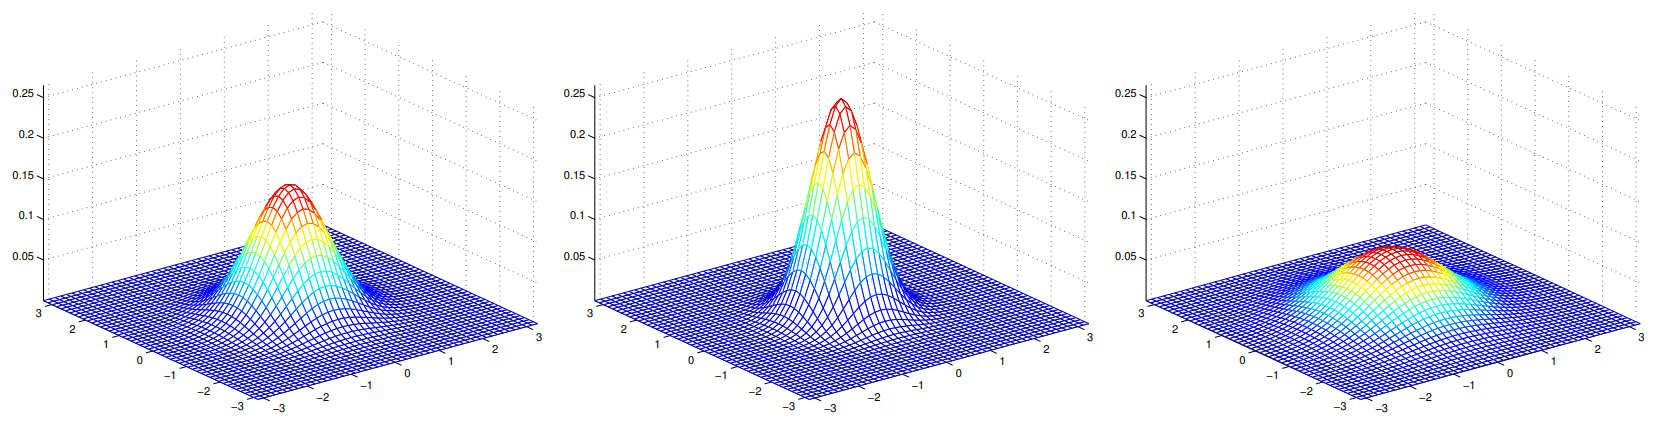
\includegraphics[width=1.0\linewidth]{figs/gaussian_density1.png}
\end{figure}

最左边的图显示的是均值为零(即 $2 \times 1$ 零向量)、协方差矩阵为 $\Sigma = I$(即 $2 \times 2$ 单位矩阵)的高斯分布。均值为零、协方差为单位矩阵的高斯分布也称为\textbf{标准正态分布}。中间的图显示的是均值为零、$\Sigma = 0.6I$ 的高斯分布的密度;最右边的图显示的是 $\Sigma = 2I$ 的高斯分布的密度。可以看到,随着 $\Sigma$ 变大,高斯分布变得更加“分散”,而随着 $\Sigma$ 变小,分布变得更加“紧凑”。

接下来看一些更多的例子。

\begin{figure}[H]
    \centering
    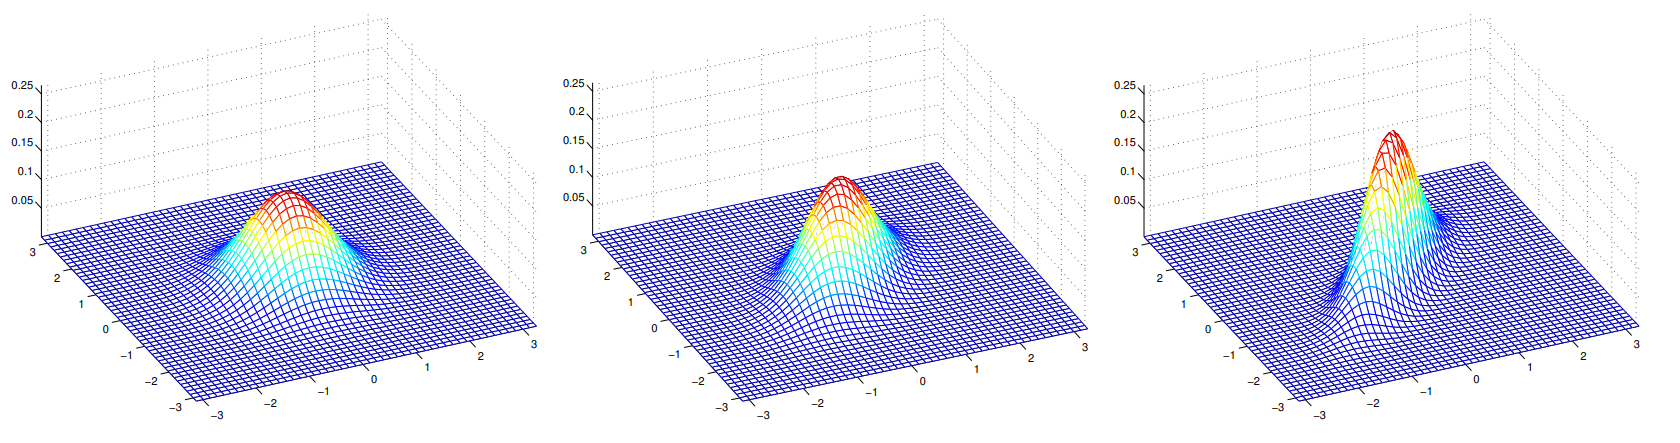
\includegraphics[width=1.0\linewidth]{figs/gaussian_density2.png}
\end{figure}

上面的图显示了均值为 0、协方差矩阵分别为
\[
    \Sigma = \begin{bmatrix} &1& &0& \\ &0& &1& \end{bmatrix}; \Sigma = \begin{bmatrix} &1& &0.5& \\ &0.5& &1& \end{bmatrix}; \Sigma = \begin{bmatrix} &1& &0.8& \\ &0.8& &1& \end{bmatrix}.
\]
最左边的图显示的是熟悉的标准正态分布,并且可以看到,随着 $\Sigma$ 中非对角线元素的增加,密度函数变得更加“压缩”到 $45^\circ$ 线(由 $x_1 = x_2$ 给出)。当观察这三个密度函数的等高线时,可以更清楚地看到这一点:

\begin{figure}[H]
    \centering
    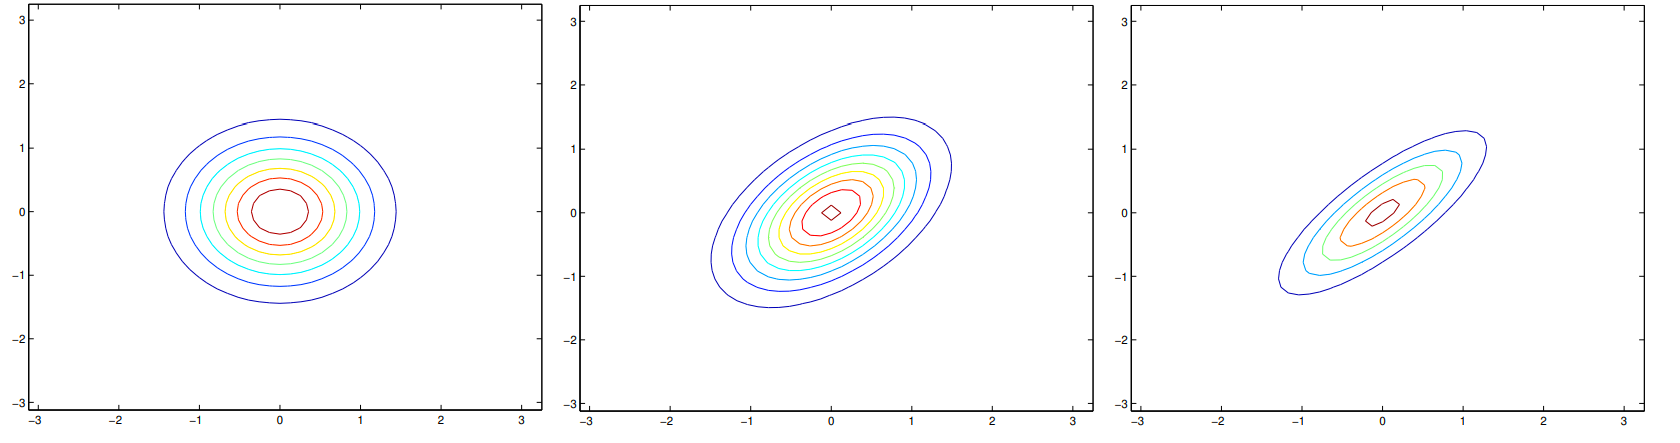
\includegraphics[width=1.0\linewidth]{figs/gaussian_contour1.png}
\end{figure}

下面是另外一组由不同的 $\Sigma$ 生成的例子:

\begin{figure}[H]
    \centering
    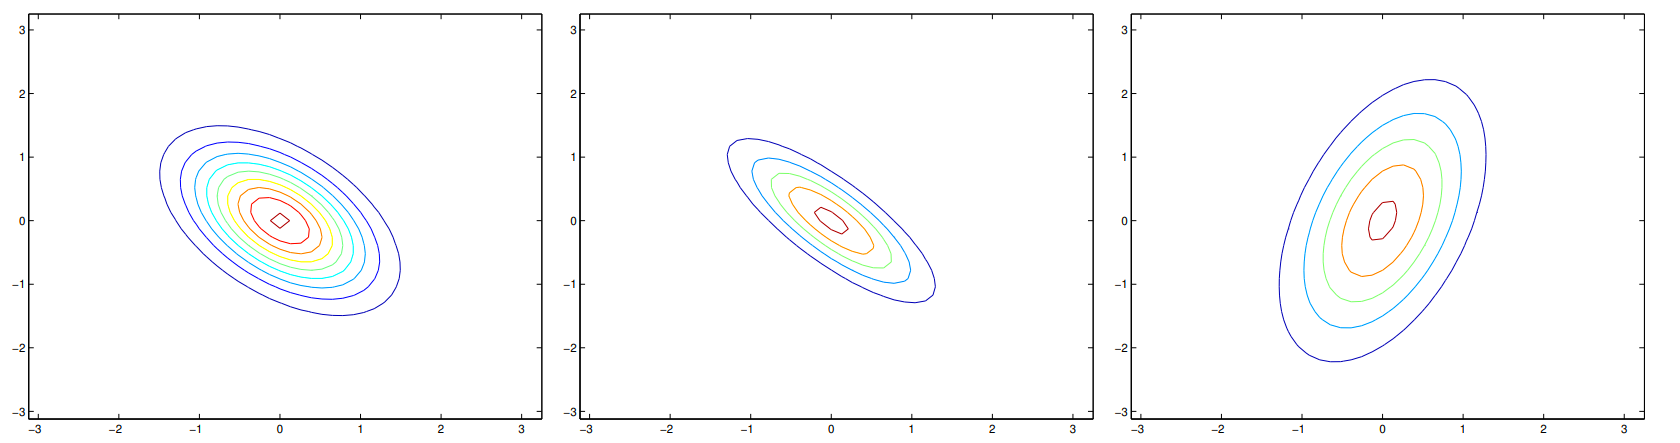
\includegraphics[width=1.0\linewidth]{figs/gaussian_contour2.png}
\end{figure}

上面的图分别使用了
\[
    \Sigma = \begin{bmatrix} &1& &-0.5& \\ &-0.5& &1& \end{bmatrix}; \Sigma = \begin{bmatrix} &1& &-0.8& \\ &-0.8& &1& \end{bmatrix}; \Sigma = \begin{bmatrix} &3& &0.8& \\ &0.8& &1& \end{bmatrix}.
\]
从最左边和中间的图可以看到,通过减小协方差矩阵的非对角线元素,密度函数再次变得“压缩”,但方向相反。最后值得一提的是,当改变参数时,等高线通常会形成椭圆(最右边的图显示了一个例子)。

作为最后一组例子,通过固定 $\Sigma = I$,并改变 $\mu$,也可以移动密度函数的均值。

\begin{figure}[H]
    \centering
    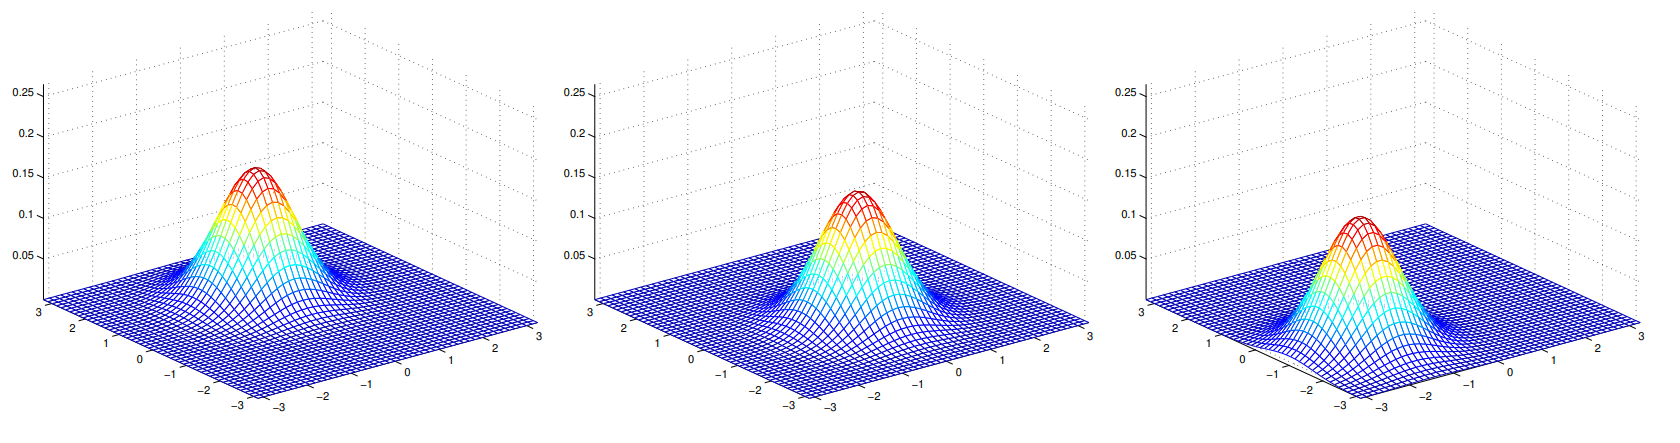
\includegraphics[width=1.0\linewidth]{figs/gaussian_density3.png}
\end{figure}

上面的图是使用 $\Sigma = I$ 生成的,并且 $\mu$ 分别为
\[
    \mu = \begin{bmatrix} &1& \\ &0& \end{bmatrix}; \mu = \begin{bmatrix} &-0.5& \\ &0& \end{bmatrix}; \mu = \begin{bmatrix} &-1& \\ &-1.5& \end{bmatrix}.
\]

\subsection{高斯判别分析模型}

当遇到输入特征 $x$ 是连续随机变量的分类问题时,可以使用高斯判别分析模型,该模型利用多元正态分布对 $p(x|y)$ 进行建模。模型如下:
\[
\begin{aligned}
    y &\sim \text{Bernoulli}(\phi) \\
    x|y=0 &\sim \mathcal{N}(\mu_0, \Sigma) \\
    x|y=1 &\sim \mathcal{N}(\mu_1, \Sigma)
\end{aligned}
\]
写出分布形式为:
\[
\begin{aligned}
    p(y) &= \phi^y (1-\phi)^{1-y} \\
    p(x|y=0) &= \frac{1}{(2\pi)^{d/2}|\Sigma|^{1/2}} \exp\left(-\frac{1}{2}(x-\mu_0)^T \Sigma^{-1} (x-\mu_0)\right) \\
    p(x|y=1) &= \frac{1}{(2\pi)^{d/2}|\Sigma|^{1/2}} \exp\left(-\frac{1}{2}(x-\mu_1)^T \Sigma^{-1} (x-\mu_1)\right)
\end{aligned}
\]
模型中的参数为 $\phi, \Sigma, \mu_0$ 和 $\mu_1$。(注意,尽管有两个不同的均值向量 $\mu_0$ 和 $\mu_1$,但该模型通常只使用一个协方差矩阵 $\Sigma$。) 数据的对数似然函数如下:
\[
\begin{aligned}
    \ell(\phi, \mu_0, \mu_1, \Sigma) &= \log \prod_{i=1}^n p(x^{(i)}, y^{(i)}; \phi, \mu_0, \mu_1, \Sigma) \\
    &= \log \prod_{i=1}^n p(x^{(i)}|y^{(i)}; \mu_0, \mu_1, \Sigma) p(y^{(i)}; \phi).
\end{aligned}
\]

通过最大化 $\ell$ 对参数进行估计,可以得到参数的最大似然估计(参见习题集 1):
\[
\begin{aligned}
    \phi &= \frac{1}{n} \sum_{i=1}^n 1\{y^{(i)} = 1\} \\
    \mu_0 &= \frac{\sum_{i=1}^n 1\{y^{(i)} = 0\}x^{(i)}}{\sum_{i=1}^n 1\{y^{(i)} = 0\}} \\
    \mu_1 &= \frac{\sum_{i=1}^n 1\{y^{(i)} = 1\}x^{(i)}}{\sum_{i=1}^n 1\{y^{(i)} = 1\}} \\
    \Sigma &= \frac{1}{n} \sum_{i=1}^n (x^{(i)} - \mu_{y^{(i)}})(x^{(i)} - \mu_{y^{(i)}})^T.
\end{aligned}
\]

从直观上看,算法的操作可以表示如下:

\begin{figure}[H]
    \centering
    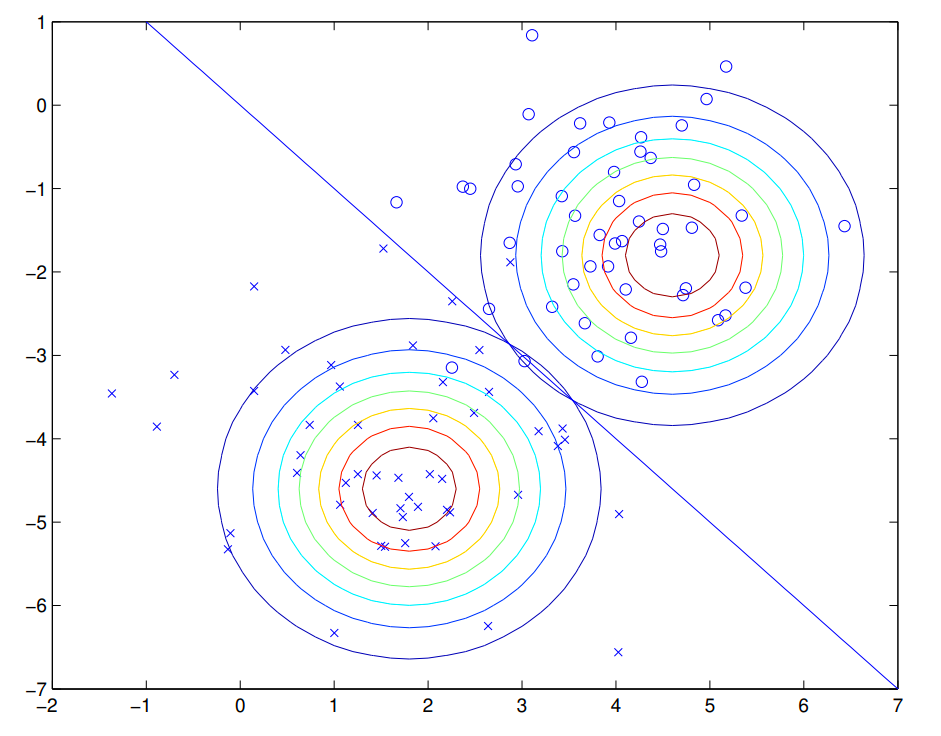
\includegraphics[width=0.5\linewidth]{figs/gda.png}
\end{figure}

图中展示了训练集以及拟合到两个类别数据的两个高斯分布的等高线。注意到由于共享协方差矩阵 $\Sigma$,这两个高斯分布的等高线形状和方向相同,但它们的均值 $\mu_0$ 和 $\mu_1$ 不同。图中还展示了 $p(y=1|x)=0.5$ 的决策边界直线。在边界的一侧,预测 $y=1$ 是最可能的结果,而在另一侧,则更多地预测 $y=0$。

\subsection{讨论:GDA 与逻辑回归}

GDA 模型与逻辑回归有着有趣的关系。如果将 $p(y=1|x; \phi, \mu_0, \mu_1, \Sigma)$ 视为 $x$ 的函数,会发现它可以表示为以下形式:
\[
    p(y=1|x; \phi, \mu_0, \mu_1, \Sigma) = \frac{1}{1+\exp(-\theta^T x)},
\]
其中 $\theta$ 是 $\phi, \mu_0, \mu_1, \Sigma$ 的适当函数。\footnote{这里采用了重新定义右侧 $x^{(i)}$ 为 $(d+1)$ 维向量的约定,即添加额外的坐标 $x_0^{(i)} = 1$;参见习题集 1。} 这正是逻辑回归(一种判别式算法)用来建模 $p(y=1|x)$ 的形式。

何时应该优先选择其中一个模型,何时又该选择另一个?GDA 和逻辑回归在同一数据集上训练时,通常会给出不同的决策边界,如何判断哪个会更好?

前文论述了,如果 $p(x|y)$ 是多元高斯分布(且共享 $\Sigma$),那么 $p(y|x)$ 必然是逻辑函数。反之则不成立,即 $p(y|x)$ 是逻辑函数并不意味着 $p(x|y)$ 是多元高斯分布。这表明 GDA 对数据做出了比逻辑回归更强的建模假设。事实证明,当这些建模假设正确时,GDA 会更好地拟合数据,并且是一个更好的模型。具体来说,当 $p(x|y)$ 确实是高斯分布(且共享 $\Sigma$)时,GDA 具有\textbf{渐近效率 (asymptotically efficient)}。非正式地讲,这意味着在训练集非常大($n$ 很大)的极限情况下,没有哪个算法能比 GDA 更好(例如,在估计 $p(y|x)$ 的准确性方面)。特别地,在这种情况下,可以证明 GDA 是比逻辑回归更好的算法;更一般地,即使训练集较小,通常也期望 GDA 表现更好。

相比之下,通过做出显著较弱的假设,逻辑回归也更\textit{鲁棒 (Robust)},对不正确的建模假设更不敏感。有许多不同的假设集合可以导致 $p(y|x)$ 呈现逻辑函数的形式。例如,如果 $x|y=0 \sim \text{Poisson}(\lambda_0)$ 且 $x|y=1 \sim \text{Poisson}(\lambda_1)$,那么 $p(y|x)$ 将是逻辑函数。逻辑回归在这种泊松分布数据上也能很好地工作。但是,如果对非高斯数据使用 GDA 并拟合高斯分布,那么结果将不太可预测,并且 GDA 可能表现不佳。

总结来说:GDA 做出了更强的建模假设,并且在建模假设正确或至少近似正确时,数据效率更高(即,需要较少的训练数据来“很好地”学习)。逻辑回归做出了较弱的假设,并且对建模假设的错误更鲁棒。具体来说,当数据确实是非高斯分布时,在大数据集的极限情况下,逻辑回归几乎总是比 GDA 表现更好。因此,在实践中,逻辑回归比 GDA 使用更频繁。(关于判别式模型与生成式模型的某些相关考虑也适用于接下来讨论的朴素贝叶斯算法,但朴素贝叶斯算法仍然被认为是一个非常好的,并且当然也是一个非常流行的分类算法。)

\section{朴素贝叶斯(选读)}

在 GDA 中,特征向量 $x$ 是连续的实值向量。接下来讨论一种不同的学习算法,其中 $x_j$ 是离散值。

以构建电子邮件垃圾邮件过滤器为例,考虑使用机器学习。希望根据消息是否为未经请求的商业(垃圾邮件)或非垃圾邮件来对其进行分类。学习完成后,可以使邮件阅读器自动过滤掉垃圾邮件,并将其放入单独的文件夹中。对电子邮件进行分类是更广泛的问题集合(称为\textbf{文本分类 (text classification)})的一个示例。

假设有一个训练集(一组标记为垃圾邮件或非垃圾邮件的电子邮件)。首先通过指定用于表示电子邮件的特征 $x_j$ 来构建垃圾邮件过滤器。

将通过一个特征向量来表示一封电子邮件,该向量的长度等于字典中的单词数量。具体来说,如果一封电子邮件包含字典中的第 $j$ 个单词,则设置 $x_j=1$;否则,设置 $x_j=0$。例如,以下向量:


\[
x = 
\begin{bmatrix}
    &1& \\
    &0& \\
    &0& \\
    &\vdots& \\
    &1& \\
    &\vdots& \\
    &0&
\end{bmatrix}
\quad % 或者 \qquad 调整间距
\begin{array}{l}
    \text{a} \\
    \text{aardvark} \\
    \text{aardwolf} \\
    \vdots \\
    \text{buy} \\
    \vdots \\
    \text{zygmurgy}
\end{array}
\]
表示一封包含单词“a”和“buy”但不包含“aardvark”、“aardwolf”或“zygmurgy”的电子邮件。\footnote{实际上,在实践中会查看训练集并仅将至少出现一次的单词编码到特征向量中,而不是查看所有英文单词的列表。除了减少建模的单词数量,从而降低计算和空间需求外,这还有一个优点,即允许对可能出现在电子邮件中(例如“cs229”)但在字典中找不到的许多单词进行建模/包含作为特征。有时(在作业中)还会排除非常高频的单词(例如“the”、“of”和“and”);这些高频的“无内容”词被称为\textbf{停用词 (stop words)},因为它们在许多文档中都会出现,并且很少能表明电子邮件是垃圾邮件还是非垃圾邮件。} 用于编码特征向量的单词集合称为\textbf{词汇表 (vocabulary)},因此 $x$ 的维度等于词汇表的大小。

在选择了特征向量之后,现在希望构建一个生成模型。因此,需要对 $p(x|y)$ 进行建模。但是,如果词汇表有 50000 个单词,那么 $x \in \{0, 1\}^{50000}$($x$ 是一个由 0 和 1 组成的 50000 维向量),如果对 $x$ 使用 2$^{50000}$ 种可能结果的多项分布进行显式建模,最终会得到一个 $(2^{50000}-1)$ 维参数向量。参数数量显然太多了。

因此,为了对 $p(x|y)$ 进行建模,将做出一个非常强的假设。假设给定 $y$ 时,$x_i$ 是条件独立的。这个假设称为\textbf{朴素贝叶斯假设 (Naive Bayes (NB) assumption)},由此产生的算法称为\textbf{朴素贝叶斯分类器 (Naive Bayes classifier)}。例如,如果 $y=1$ 表示垃圾邮件,“buy”是第 2087 个单词,“price”是第 39831 个单词;那么假设如果知道 $y=1$(这封特定的电子邮件是垃圾邮件),那么关于 $x_{2087}$ 的知识(消息中是否出现“buy”)对关于 $x_{39831}$ 的值(是否出现“price”)的信念没有影响。更正式地讲,这可以写成 $p(x_{2087}|y) = p(x_{2087}|y, x_{39831})$。(注意,这与 $x_{2087}$ 和 $x_{39831}$ 是独立的说法不同,独立的说法会写成 $p(x_{2087}) = p(x_{2087}|x_{39831})$;相反,这里只假设给定 $y$ 时,$x_{2087}$ 和 $x_{39831}$ 是条件独立的。)

现在有:
\[
    \begin{aligned}
        p(x_1, \dots, x_{50000}|y) &= p(x_1|y)p(x_2|y, x_1)p(x_3|y, x_1, x_2) \cdots p(x_{50000}|y, x_1, \dots, x_{49999}) \\ 
        &= p(x_1|y)p(x_2|y)p(x_3|y) \cdots p(x_{50000}|y) \\ 
        &= \prod_{j=1}^d p(x_j|y) 
    \end{aligned}
\]
第一个等号仅遵循概率的通常性质,第二个等号使用了朴素贝叶斯假设。注意,尽管朴素贝叶斯假设是一个非常强的假设,但由此产生的算法在许多问题上效果很好。

模型由 $\phi_{j|y=1} = p(x_j=1|y=1)$、$\phi_{j|y=0} = p(x_j=1|y=0)$ 和 $\phi_y = p(y=1)$ 参数化。像往常一样,给定训练集 $\{(x^{(i)}, y^{(i)}); i=1, \dots, n\}$,可以写出数据的联合似然:
\[
    \mathcal{L}(\phi_y, \phi_{j|y=0}, \phi_{j|y=1}) = \prod_{i=1}^n p(x^{(i)}, y^{(i)}).
\]
关于 $\phi_y$、$\phi_{j|y=0}$ 和 $\phi_{j|y=1}$ 最大化此式,得到最大似然估计:
\[
    \begin{aligned}
        \phi_{j|y=1} &= \frac{\sum_{i=1}^n {1}\{x_j^{(i)} = 1 \wedge y^{(i)} = 1\}}{\sum_{i=1}^n {1}\{y^{(i)} = 1\}} \\ 
        \phi_{j|y=0} &= \frac{\sum_{i=1}^n {1}\{x_j^{(i)} = 1 \wedge y^{(i)} = 0\}}{\sum_{i=1}^n {1}\{y^{(i)} = 0\}} \\ 
        \phi_y &= \frac{\sum_{i=1}^n {1}\{y^{(i)} = 1\}}{n} 
    \end{aligned}
\]
在上面的公式中,“$\wedge$”符号表示“逻辑且”。参数具有非常自然的解释。例如,$\phi_{j|y=1}$ 是单词 $j$ 出现在垃圾邮件 ($y=1$) 中的比例。

在拟合了所有这些参数之后,为了对具有特征 $x$ 的新示例进行预测,只需计算:
\[
\begin{aligned}
    p(y=1|x) &= \frac{p(x|y=1)p(y=1)}{p(x)} \\
    &= \frac{\left(\prod_{j=1}^d p(x_j|y=1)\right) p(y=1)}{\left(\prod_{j=1}^d p(x_j|y=1)\right) p(y=1) + \left(\prod_{j=1}^d p(x_j|y=0)\right) p(y=0)},
\end{aligned}
\]
并选择后验概率较高的类别。

最后,注意,虽然主要针对特征 $x_j$ 是二值的问题开发了朴素贝叶斯算法,但可以很直接地将其推广到 $x_j$ 可以取 $\{1, 2, \dots, k_j\}$ 中的值,只需将 $p(x_j|y)$ 建模为多项分布而不是伯努利分布。实际上,即使某些原始输入属性(例如,之前示例中的房屋居住面积)是连续值,通常也会将其\textbf{离散化 (discretize)}——即将其转换为一小组离散值,然后应用朴素贝叶斯。例如,如果使用某个特征 $x_j$ 来表示居住面积,可以将连续值离散化如下:

\begin{table}[H]
    \centering
    \begin{tabular}{c|c|c|c|c|c}
        居住面积 (平方英尺) & < 400 & 400-800 & 800-1200 & 1200-1600 & > 1600 \\
        \hline
        $x_i$ & 1 & 2 & 3 & 4 & 5 
    \end{tabular}
\end{table}

因此,对于居住面积为 890 平方英尺的房屋,可以将相应的特征 $x_j$ 的值设置为 3。然后可以应用朴素贝叶斯算法,并如前所述,使用多项分布对 $p(x_j|y)$ 进行建模。当原始的连续值属性无法通过多元正态分布很好地建模时,离散化特征并使用朴素贝叶斯(而不是 GDA)通常会产生更好的分类器。

\subsection{拉普拉斯平滑}

如前所述,朴素贝叶斯算法在许多问题上效果相当不错,但有一个简单的修改可以使其效果更好,尤其是在文本分类方面。简要讨论一下该算法当前形式存在的问题,然后讨论如何解决它。

考虑垃圾邮件/电子邮件分类,假设于 20xx 年,在您 CS229 结课并出色地完成了项目后,您决定在 20xx 年 5 月左右提交您的工作以在 NeurIPS 会议上发表。\footnote{NeurIPS 是顶级机器学习会议之一。提交论文的截止日期通常在五月至六月。} 因为会在电子邮件中讨论该会议,所以您也开始收到包含“neurips”一词的消息。但这是您的第一篇 NeurIPS 论文,在此之前,您从未见过包含“neurips”一词的电子邮件;特别是在垃圾邮件/非垃圾邮件训练集中,“neurips”从未出现过。假设“neurips”是字典中的第 35000 个单词,您的朴素贝叶斯垃圾邮件过滤器会选择其最大似然估计参数 $\phi_{35000|y}$ 为:

\begin{align*} 
\phi_{35000|y=1} &= \frac{\sum_{i=1}^n {1}\{x_{35000}^{(i)} = 1 \wedge y^{(i)} = 1\}}{\sum_{i=1}^n {1}\{y^{(i)} = 1\}} = 0 \\ \phi_{35000|y=0} &= \frac{\sum_{i=1}^n {1}\{x_{35000}^{(i)} = 1 \wedge y^{(i)} = 0\}}{\sum_{i=1}^n {1}\{y^{(i)} = 0\}} = 0 
\end{align*}
也就是说,由于它从未在垃圾邮件或非垃圾邮件训练示例中见过“neurips”,它认为在任何类型的电子邮件中看到它的概率为零。因此,当尝试判断这些包含“neurips”的消息是否是垃圾邮件时,它会计算类别后验概率,并得到
\[
    p(y=1|x) = \frac{\prod_{j=1}^d p(x_j|y=1) p(y=1)}{\prod_{j=1}^d p(x_j|y=1) p(y=1) + \prod_{j=1}^d p(x_j|y=0) p(y=0)} = \frac{0}{0}.
\]
这是因为 $\prod_{j=1}^d p(x_j|y)$ 的每一项都包含一个 $p(x_{35000}|y) = 0$ 的项,该项与乘积相乘。因此,算法得到 0/0,无法做出预测。

更广泛地说,仅仅因为在有限的训练集中没有看到某个事件,就将其概率估计为零,这在统计上是一个糟糕的主意。考虑估计一个多项随机变量 $z$ 取值为 $\{1, \dots, k\}$ 的问题。可以用 $\phi_j = p(z=j)$ 参数化多项分布。给定一组 $n$ 个独立观测值 $\{z^{(1)}, \dots, z^{(n)}\}$,最大似然估计由下式给出:
\[
    \phi_j = \frac{\sum_{i=1}^n {1}\{z^{(i)} = j\}}{n}.
\]
正如之前看到的,如果使用这些最大似然估计,那么一些 $\phi_j$ 可能会变为零,这是一个问题。为了避免这种情况,可以使用\textbf{拉普拉斯平滑 (Laplace smoothing)},它将上述估计替换为:
\[
    \phi_j = \frac{1 + \sum_{i=1}^n {1}\{z^{(i)} = j\}}{k + n}.
\]
在这里,在分子中加了 1,在分母中加了 $k$。注意,$\sum_{j=1}^k \phi_j = 1$ 仍然成立(自己验证一下!),这是一个理想的属性,因为 $\phi_j$ 是概率的估计,而概率之和必须为 1。此外,对于所有 $j$ 的值,$\phi_j \ne 0$,解决了概率估计为零的问题。在某些(可以说相当强的)条件下,可以证明拉普拉斯平滑实际上给出了 $\phi_j$ 的最优估计。

回到朴素贝叶斯分类器,使用拉普拉斯平滑,因此得到以下参数估计:
\begin{align*} \phi_{j|y=1} &= \frac{1 + \sum_{i=1}^n {1}\{x_j^{(i)} = 1 \wedge y^{(i)} = 1\}}{2 + \sum_{i=1}^n {1}\{y^{(i)} = 1\}} \\ \phi_{j|y=0} &= \frac{1 + \sum_{i=1}^n {1}\{x_j^{(i)} = 1 \wedge y^{(i)} = 0\}}{2 + \sum_{i=1}^n {1}\{y^{(i)} = 0\}} \end{align*}
(在实践中,是否对 $\phi_y$ 应用拉普拉斯平滑通常无关紧要,因为通常垃圾邮件和非垃圾邮件的比例都相当可观,所以 $\phi_y$ 将是 $p(y=1)$ 的合理估计,并且无论如何都会远离 0。)

\subsection{文本分类的事件模型}

为了结束关于生成学习算法的讨论,下面讨论一个专门用于文本分类的模型。虽然前面介绍的朴素贝叶斯在许多分类问题上效果很好,但对于文本分类,有一个相关的模型效果更好。

在文本分类的具体背景下,前面介绍的朴素贝叶斯使用了\textbf{伯努利事件模型 (Bernoulli event model)}(或有时称为\textbf{多元伯努利事件模型 (multi-variate Bernoulli event model)})。在该模型中,假设生成电子邮件的过程是:首先随机确定(根据类别先验 $p(y)$)发送者是垃圾邮件发送者还是非垃圾邮件发送者。然后,发送电子邮件的人遍历字典,独立地决定是否根据概率 $p(x_j=1|y) = \phi_{j|y}$ 在该电子邮件中包含每个单词 $j$。因此,消息的概率由 $p(y) \prod_{j=1}^d p(x_j|y)$ 给出。

这里有一个不同的模型,称为\textbf{多项事件模型 (Multinomial event model)}。为了描述该模型,将使用不同的表示法和特征集来表示电子邮件。令 $x_j$ 表示电子邮件中第 $j$ 个单词的标识。因此,$x_j$ 现在是一个整数,取值范围为 $\{1, \dots, |V|\}$,其中 $|V|$ 是词汇表(字典)的大小。包含 $d$ 个单词的电子邮件现在由一个长度为 $d$ 的向量 $(x_1, x_2, \dots, x_d)$ 表示;注意 $d$ 可以因不同的文档而异。例如,如果一封电子邮件以“A NeurIPS ...”开头,那么 $x_1=1$(“a”是字典中的第一个单词),$x_2=35000$(如果“neurips”是字典中的第 35000 个单词)。

在多项事件模型中,假设生成电子邮件的过程是一个随机过程,其中首先确定(根据 $p(y)$)是垃圾邮件还是非垃圾邮件,这与之前相同。然后,发送电子邮件的人通过首先从某个多项分布 $p(x_1|y)$ 生成 $x_1$ 来编写电子邮件。接下来,第二个单词 $x_2$ 独立于 $x_1$ 但来自相同的多项分布中选择,对于 $x_3, x_4$ 等也是如此,直到生成了电子邮件中的所有 $d$ 个单词。因此,消息的总概率由 $p(y) \prod_{j=1}^d p(x_j|y)$ 给出。注意,该公式看起来与之前在伯努利事件模型下消息概率的公式相同,但公式中的项现在表示完全不同的事物。特别是 $p(x_j|y)$ 现在是一个多项分布而非伯努利分布。

新模型的参数是 $\phi_y = p(y)$ 和 $\phi_{k|y=1} = p(x_j = k | y = 1)$(对于任何 $j$)以及 $\phi_{k|y=0} = p(x_j = k | y = 0)$。注意,假设 $p(x_j|y)$ 对于所有 $j$ 的值都是相同的(即,生成单词的分布不依赖于它在电子邮件中的位置 $j$)。

如果给定训练集 $\{(x^{(i)}, y^{(i)}); i=1, \dots, n\}$,其中 $x^{(i)} = (x_1^{(i)}, x_2^{(i)}, \dots, x_{d_i}^{(i)})$(此处,$d_i$ 是第 $i$ 个训练样本中的单词数),则数据的似然由下式给出:
\begin{align*}
    \mathcal{L}(\phi_y, \phi_{k|y=0}, \phi_{k|y=1}) &= \prod_{i=1}^n p(x^{(i)}, y^{(i)})\\
    &= \prod_{i=1}^n \left( \prod_{j=1}^{d_i} p(x_j^{(i)} | y^{(i)}; \phi_{k|y=0}, \phi_{k|y=1}) \right) p(y^{(i)}; \phi_y).
\end{align*}

最大化此似然得到参数的最大似然估计:
\begin{align*} 
    \phi_{k|y=1} &= \frac{\sum_{i=1}^n \sum_{j=1}^{d_i} {1}\{x_j^{(i)} = k \wedge y^{(i)} = 1\}}{\sum_{i=1}^n {1}\{y^{(i)} = 1\} d_i} \\ 
    \phi_{k|y=0} &= \frac{\sum_{i=1}^n \sum_{j=1}^{d_i} {1}\{x_j^{(i)} = k \wedge y^{(i)} = 0\}}{\sum_{i=1}^n {1}\{y^{(i)} = 0\} d_i} \\ 
    \phi_y &= \frac{\sum_{i=1}^n {1}\{y^{(i)} = 1\}}{n}. 
\end{align*}
如果对估计 $\phi_{k|y=0}$ 和 $\phi_{k|y=1}$ 应用拉普拉斯平滑(在实践中为了获得良好性能是必需的),在分子中加 1,在分母中加 $|V|$,得到:
\begin{align*} 
    \phi_{k|y=1} &= \frac{1 + \sum_{i=1}^n \sum_{j=1}^{d_i} {1}\{x_j^{(i)} = k \wedge y^{(i)} = 1\}}{|V| + \sum_{i=1}^n {1}\{y^{(i)} = 1\} d_i} \\ 
    \phi_{k|y=0} &= \frac{1 + \sum_{i=1}^n \sum_{j=1}^{d_i} {1}\{x_j^{(i)} = k \wedge y^{(i)} = 0\}}{|V| + \sum_{i=1}^n {1}\{y^{(i)} = 0\} d_i}. 
\end{align*}
虽然朴素贝叶斯分类器不一定是最好的分类算法,但它通常效果出奇地好。考虑到其简单性和易于实现性,它通常也是一个非常好的“第一步”尝试。